\documentclass[
    ngerman,
    accentcolor=TUDa-1c,
    % dark_mode,
    fontsize= 12pt,
    a4paper,
    aspectratio=169,
    colorback=true,
    fancy_row_colors,
    leqno,
    fleqn,
    boxarc=3pt,
    fleqn,
    % shell_escape = false, % Kompatibilität mit sharelatex
    ]{algoslides}

%%------------%%
%%--Packages--%%
%%------------%%

% \usepackage{audutils}
% \usepackage{fopbot}
\usepackage{booktabs}
\usepackage{tikz}
\usetikzlibrary{3d, angles, animations, arrows, arrows.meta, arrows.spaced, automata, babel, backgrounds, bending, calc, calendar, chains, circuits.ee.IEC, circuits.logic.CDH, circuits.logic.IEC, circuits.logic.US, datavisualization, datavisualization.formats.functions, datavisualization.polar, decorations, decorations.footprints, decorations.fractals, decorations.markings, decorations.pathmorphing, decorations.pathreplacing, decorations.shapes, decorations.text, er, external, fadings, fit, fixedpointarithmetic, folding, fpu, graphs, graphs.standard, intersections, lindenmayersystems, math, matrix, patterns, patterns.meta, perspective, petri, plotmarks, positioning, quotes, rdf, scopes, shadings, shadows, shadows.blur, shapes, shapes.arrows, shapes.callouts, shapes.gates.logic.IEC, shapes.gates.logic.US, shapes.geometric, shapes.misc, shapes.multipart, shapes.symbols, spy, svg.path, through, tikzmark, topaths, trees, turtle, views}

\tikzset{%
    node/.style={rectangle, text=white, fill=TUDa-0c, very thick, minimum width=8em, minimum height=2em},
    node_s/.style={node, minimum width=6em},
    commit/.style={node_s, fill=accentcolor, text=white},
    mergecommit/.style={commit, fill=accentcolor!50, text=white},
    head/.style={
        rounded corners=1em,
        node_s,
        fill=TUDa-8b,
        append after command={
            (\tikzlastnode.center) node[text=white] {\texttt{HEAD}}
        }
    },
    branch/.style={
        rounded corners=1em,
        node_s,
        fill=TUDa-4c
    },
    node9/.style={rectangle, rounded corners=1em, text=white, fill=TUDa-9b, very thick, minimum width=8em, minimum height=2em},
    arc/.style={-Latex, thick},
    node_inactive/.style={rectangle, rounded corners=1em, text=white, fill=TUDa-0a, very thick, minimum width=8em, minimum height=2em},
    arc_inactive/.style={-Latex, thick, draw=TUDa-0a, text=TUDa-0a},
    square/.style={minimum width=5em, minimum height=5em},
    box/.style={node_inactive, rounded corners=1em}
}

% Import all Packages from Main Preamble with relative Path (buggy, list packages instead)
% \subimport*{../../}{preamble}

%%--------------------------%%
%%--Imports from Main File--%%
%%--------------------------%%

% Get Labels from Main Document using the xr-hyper Package
\externaldocument[ext:]{../main}
% Set Graphics Path, so pictures load correctly
\graphicspath{{../pictures}}

\begin{document}

\section{Was ist Git?}
\begin{frame}[c]
    \centering
    \Large
    \textbf{Was ist Git?}
\end{frame}

\section{Commits}

\begin{frame}
    \slidehead
    \begin{itemize}
        \item Datei hinzugefügt, geändert, verschoben oder gelöscht
        \item mit Nachricht versehen
        \item \enquote{kryptische} Bezeichnung (Hash), z.B. \texttt{bc7f1a9e22bc7f19e22bc}\dots
        \begin{itemize}
            \item erste fünf Zeichen zur Identifizierung meist ausreichend
        \end{itemize}
    \end{itemize}
\end{frame}

\begin{frame}
    \slidehead
    \vspace{-1em}
    \centering
    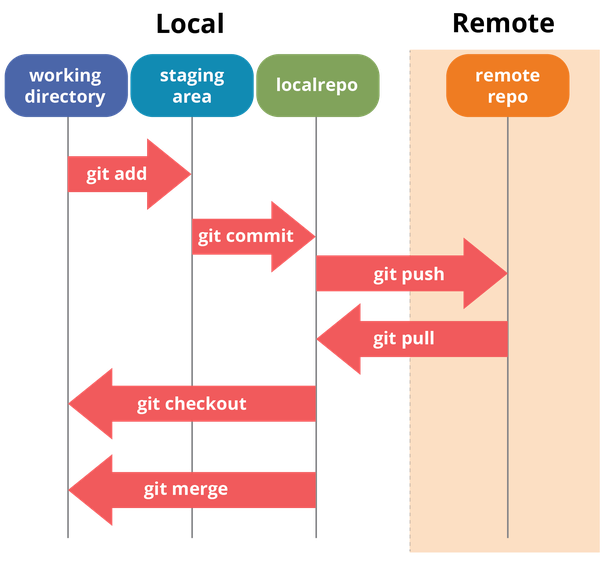
\includegraphics[scale=.3]{../pictures/structure-overview.png}
\end{frame}

\begin{frame}
    \slidehead
    \vspace{1em}
    \centering
    \begin{tikzpicture}
        % state 1
        \node[commit](c1){c1c1c};
        \node<1>[head, below=2 em of c1](head0){};
        \draw<1>[arc] (head0) to (c1);
        % state 2
        \node<2->[commit, right=2 em of c1](c2){c2c2c};
        \draw<2->[arc] (c2) to (c1);
        \node<2>[head, below=2 em of c2](head1){};
        \draw<2>[arc] (head1) to (c2);
        % state 3
        \node<3->[commit, right=2 em of c2](c3){c3c3c};
        \draw<3->[arc] (c3) to (c2);
        \node<3>[head, below=2 em of c3](head2){};
        \draw<3>[arc] (head2) to (c3);
        % state 4
        \node<4->[branch, below=2em of c3](branch_master){master};
        \draw<4->[arc] (branch_master) to (c3);
        \node<4>[head, below=2em of branch_master](head2){};
        \draw<4>[arc] (head2) to (branch_master);
        % state 5
        \node<5->[head, below=2em of c2](head2){};
        \draw<5->[arc] (head2) to (c2);
    \end{tikzpicture}
    \vspace{1em}\par
    \only<1>{initialer Commit \texttt{c1c1c}, z.B. \texttt{"initial commit"}}
    \only<2>{Commit \texttt{c2c2c}, z.B. \texttt{"implement add and mul"}}
    \only<3>{Commit \texttt{c3c3c}, z.B. \texttt{"fix sum"}}
    \only<4>{\texttt{HEAD} zeigt \textit{indirekt} auf einen Commit (hier \texttt{c3c3c})}
    \only<5>{\texttt{HEAD} kann auch \textit{direkt} auf Commit (hier \texttt{c2c2c}) zeigen}
\end{frame}

\section{Staging}

\begin{frame}[c]
    \slidehead
    \center
    \begin{tikzpicture}
        \node[node_inactive] (untracked) {untracked};
        \node[node_inactive, below=2.5em of untracked] (staged) {staged};
        \node[node_inactive, below=2.5em of staged] (unmodified) {unmodified};
        \node[node_inactive, below=2.5em of unmodified] (modified) {modified};
        \draw[arc_inactive] (untracked.south) -- (staged.north) node[right, pos=0.5] {\texttt{git add}};
        \draw[arc_inactive] (staged.south) -- (unmodified.north) node[right, pos=0.5] {\texttt{git commit}};
        \draw[arc_inactive] (unmodified.south) -- (modified.north) node[right, pos=.5] {Ändern};
        \draw[arc_inactive] (modified) to[out=180, in=180, looseness=1.5] node[left, pos=.5] {Ändern} (staged);
        \draw[arc_inactive] (modified) to[out=0,in=0, looseness=1.5] node[right, pos=.5] {\texttt{git rm}} (untracked);
        \node<7,2,3,6>[node] (untracked) {untracked};
        \node<7,3,4,6>[node, below=2.5em of untracked] (staged) {staged};
        \node<7,4,5>[node, below=2.5em of staged] (unmodified) {unmodified};
        \node<7,5,6>[node, below=2.5em of unmodified] (modified) {modified};
        \draw<7,3>[arc] (untracked.south) -- (staged.north) node[right, pos=0.5] {\texttt{git add}};
        \draw<7,4>[arc] (staged.south) -- (unmodified.north) node[right, pos=0.5] {\texttt{git commit}};
        \draw<7,5>[arc] (unmodified.south) -- (modified.north) node[right, pos=.5] {Ändern};
        \draw<7,6>[arc] (modified) to[out=180, in=180, looseness=1.5] node[left, pos=.5] {Ändern} (staged);
        \draw<7,6>[arc] (modified) to[out=0,in=0, looseness=1.5] node[right, pos=.5] {\texttt{git rm}} (untracked);
    \end{tikzpicture}
\end{frame}

\section{Branches}

\begin{frame}[c]
    \slidehead
    \centering
    \begin{tikzpicture}
        % state 1
        \node<1->[commit](c0){c0c0c};
        \node<1->[commit, right=2em of c0](c1){c1c1c};
        \node<1-2>[branch, right=2em of c1](bm1){master};
        \draw<1->[arc] (c1) to (c0);
        \draw<1-2>[arc] (bm1) to (c1);
        % state 2
        \node<2-3>[branch, below=1em of bm1](fa1){feature};
        \draw<2-3>[arc] (fa1.west) to (c1.east);
        % state 3
        \node<3->[commit, right=2em of c1](c2){c2c2c};
        \node<3->[branch, right=2em of c2](bm2){master};
        \draw<3->[arc] (c2) to (c1);
        \draw<3->[arc] (bm2) to (c2);
        % state 4
        \node<4->[commit, below=1em of c2](c3){c3c3c};
        \node<4>[branch, right=2em of c3](fa2){feature};
        \node<4->[branch, right=2em of c2](bm3){master};
        \draw<4->[arc] (c3.west) to (c1.east);
        \draw<4->[arc] (fa2) to (c3);
        % state 5
        \node<5->[commit, right=2em of c3](c4){c4c4c};
        \node<5->[branch, right=2em of c4](fa3){feature};
        \draw<5->[arc] (fa3) to (c4);
    \end{tikzpicture}
    \vspace{1em}\par
    \begin{enumerate}
        \item<1->{\texttt{master}-Branch verweist auf Commit \texttt{c1c1c}}
        \item<2->{\texttt{feature}-Branch wird von \texttt{master}-Branch abgeleitet}
        \item<3->{neuer Commit \texttt{c2c2c} in \texttt{master}-Branch}
        \item<4->{neuer Commit \texttt{c3c3c} in \texttt{feature}-Branch}
        \item<5->{neuer Commit \texttt{c4c4c} in \texttt{feature}-Branch}
    \end{enumerate}
\end{frame}

\section{Merging}

\begin{frame}[c]
    \centering
    \Large
    \textbf{Wie gelangen die Commits von einen Branch in einen anderen?}
\end{frame}

\subsection*{Fast-Forward Merge}

\begin{frame}[c]
    \slidehead
    \centering
    \begin{tikzpicture}
        % create c1
        \node<1->[commit](c1){c1c1c} node[left=1em of c1]{$\dots$};
        % create master
        \node<1-1>[branch, right=2em of c1](m1){master};
        \draw<1-1>[arc] (m1) to (c1);
        % create c2
        \node<1->[commit, below=1em of m1](c2){c2c2c};
        \draw<1->[arc] (c2.west) to (c1.east);
        % create c3
        \node<1->[commit, right=2em of c2](c3){c3c3c};
        \draw<1->[arc] (c3) to (c2);
        % create branch feature
        \node<1->[branch, right=2em of c3](fa1){feature};
        \draw<1->[arc] (fa1) to (c3);
        % 2 # create master
        \node<2->[branch, above=1em of fa1](m2){master};
        \draw<2->[arc] (m2.west) to (c3.east);
    \end{tikzpicture}
    \vspace{2em}
    \begin{itemize}
        \item \textbf{Fast-Forward Merge}
        \item möglich, wenn zu mergende Branches \textit{nicht} divergiert
        \item<2-> lässt \texttt{master}-Branch \textit{direkt} auf Commit von \texttt{feature}-Branch zeigen
        \item<2-> \textit{kein} Merge-Commit notwendig (gleich mehr)
        \item<3-> einfachster Fall, aber seltener
    \end{itemize}
\end{frame}

\subsection*{Normalfall}

\begin{frame}
    \slidehead
    \centering
    \vspace{2em}\par
    \begin{tikzpicture}
        % create c1
        \node<1->[commit](c1){c1c1c} node[left=1em of c1]{$\dots$};
        % create c3
        \node<1->[commit, right=2em of c1](c3){c3c3c};
        \draw<1->[arc] (c3) to (c1);
        % create master 1
        \node<1>[branch, right=2em of c3](m1){master};
        \draw<1>[arc] (m1) to (c3);
        % create c2
        \node<1->[commit, below=1em of c3](c2){c2c2c};
        \draw<1->[arc] (c2.west) to (c1.east);
        % create c4
        \node<1->[commit, right=2em of c2](c4){c4c4c};
        \draw<1->[arc] (c4) to (c2);
        % create branch feature
        \node<1->[branch, right=2em of c4](fa1){feature};
        \draw<1->[arc] (fa1) to (c4);
        % create c5
        \node<2->[mergecommit, above=1em of fa1](c5){c5c5c};
        \draw<2->[arc] (c5) to (c3);
        \draw<2->[arc] (c5.west) to (c4.east);
        % create master 2
        \node<2->[branch, right=2em of c5](m){master};
        \draw<2->[arc] (m) to (c5);

    \end{tikzpicture}
    \vspace{2em}
    \begin{itemize}
        \item \textbf{Normalfall}
        \item \texttt{master}-Branch und \texttt{feature}-Branch sind divergiert
        \item<2-> Commit \texttt{c5c5c} ist Merge-Commit aus \texttt{master}- und \texttt{feature}-Branch
    \end{itemize}
\end{frame}


\subsection*{Normalfall mit Squash}

\begin{frame}
    \slidehead
    \centering

    \begin{tikzpicture}
        % create c1
        \node<1->[commit](c1){c1c1c} node[left=1em of c1]{$\dots$};
        % create c3
        \node<1->[commit, right=2em of c1](c3){c3c3c};
        \draw<1->[arc] (c3) to (c1);
        % create master 1
        \node<1>[branch, right=2em of c3](m1){master};
        \draw<1>[arc] (m1) to (c3);
        % create c2
        \node<1>[commit, below=2em of c3](c2){c2c2c};
        \draw<1>[arc] (c2.west) to (c1.east);
        % create c4
        \node<1>[commit, right=2em of c2](c4){c4c4c};
        \draw<1>[arc] (c4) to (c2);
        % create branch feature
        \node<1>[branch, right=2em of c4](fa1){feature};
        \draw<1>[arc] (fa1) to (c4);
        % 2 # create c5
        \node<2->[mergecommit, below right=1.5em and 2em of c1, minimum width=14em](c5){c5c5c};
        \draw<2->[arc] (c5.west) to (c1.east);
        % 2 # create c2
        \node<2->[commit, below right=5em and 2em of c1](c2){c2c2c};
        \draw<2->[arc] (c2.west) to (c1.east);
        % 2 # create c4
        \node<2->[commit, right=2em of c2](c4){c4c4c};
        \draw<2->[arc] (c4) to (c2);
        % 2 # create c6
        \node<2->[mergecommit, right=10em of c3](c6){c6c6c};
        \draw<2->[arc] (c6) to (c3);
        \draw<2->[arc] (c6.west) to (c5.east);
        % 2 # create branch feature
        \node<2->[branch, right=2em of c4](fa1){feature};
        \draw<2->[arc] (fa1) to (c4);
        % 2 # create branch master
        \node<2->[branch, right=2em of c6](m){master};
        \draw<2->[arc] (m) to (c6);
        % create meta
        % \draw<2->[arc, dotted] ([yshift=1.5em] c2.north) to (c2.north);
        \draw<2->[arc, dotted] ([yshift=1.5em] c4.north) to (c4.north);
    \end{tikzpicture}
    \vspace{1em}
    \begin{itemize}
        \item \textbf{Normalfall mit Squash} (optional)
        \item<2-> Commit \texttt{c5c5c} ist Zusammenfassung des \texttt{feature}-Branches
        \item<2-> Commits \texttt{c2c2c} und \texttt{c4c4c} in Commit \texttt{c5c5c} nicht mehr sichtbar
    \end{itemize}
\end{frame}

\subsection*{Merge Conflicts}
\begin{frame}[fragile, c]
    \slidehead
    \vspace{1em}
    \begin{codeBlock}[]{minted language=java}
        public static void mul(int a, int b) {
        <<<<<<< HEAD:Calculator.java
            return a * b;
        =======
            for (int i = 0; i < b; i++) {
                a += a;
            }
        >>>>>>> feature:Calculator.java
        }
    \end{codeBlock}
\end{frame}

\section{Rebasing}

\begin{frame}
    \slidehead
    \centering
    \vspace{1em}
    \begin{tikzpicture}
        % 1 # create c1
        \node<1->[commit](c1){c1c1c} node[left=1em of c1]{$\dots$};
        % 1 # create master 1
        \node<1>[branch, right=2em of c1](m1){master};
        \draw<1>[arc] (m1) to (c1);
        % 1 # create c2
        \node<1-2>[commit, below=1em of m1](c2){c2c2c};
        \draw<1-2>[arc] (c2.west) to (c1.east);
        % 1 # create feature
        \node<1-2>[branch, right=2em of c2](fa1){feature};
        \draw<1-2>[arc] (fa1) to (c2);
        % 2 # create c3
        \node<2->[commit, right=2em of c1](c2){c3c3c};
        \draw<2->[arc] (c2.west) to (c1.east);
        % 2 # create master 2
        \node<2->[branch, right=2em of c3](m1){master};
        \draw<2->[arc] (m1) to (c3);
        % 3 # create c2
        \node<3->[commit, below=1em of m1](c2){c2c2c};
        \draw<3->[arc] (c2.west) to (c3.east);
        % 3 # create feature
        \node<3->[branch, right=2em of c2](fa1){feature};
        \draw<3->[arc] (fa1) to (c2);
    \end{tikzpicture}
    \vspace{1em}
    \begin{itemize}
        \item<2-> neuer Commit \texttt{c3c3c} auf \texttt{master}-branch
        \item<2-> Annahme: Commit \texttt{c3c3c} ist zur Weiterarbeit auf \texttt{feature}-Branch nötig
        \item<3-> \textbf{Rebase} ändert Base des ersten Commits auf \texttt{feature}-Branch
    \end{itemize}
\end{frame}

\section{Remote und Local}
\begin{frame}[c]
    \slidehead
    \center
    \begin{tikzpicture}
        \node[node, square] (server) {Remote};
        \node[node, square, right=8em of server] (client) {Local};
        \draw[arc] (server) to[out=90, in=90, looseness=.5] node[above]{\texttt{fetch}} (client);
        \draw[arc] (client) to[out=270, in=270, looseness=.5] node[below]{\texttt{push}} (server);
    \end{tikzpicture}
\end{frame}

\section{GitLab}

\begin{frame}[c]
    \centering
    \Large
    \textbf{GitLab}
\end{frame}

\section{Good and Bad Practices}

\begin{frame}{Bad Practices}
    \slidehead
    \begin{itemize}
        \item Arbeiten auf dem \texttt{master}-Branch
        \item Veröffentlichen von sensiblen Daten
        \item Unfokusierte commits
        \item git pull mit auto merge
        \item Force push
        \item Comitting binaries (mit ausnahmen)
        \item Large files (use git LFS)
    \end{itemize}
\end{frame}

\section{Live Giting}

\end{document}
